\subsection{Development of the LHC-MKI Beam Screen}
\label{sec:mki-screen-development}

During the commissioning of the CERN accelerator complex for LHC type beam with 25ns, 50ns and 75ns bunch spacing, drastic heating and outgassing was observed in the SPS extraction kicker magnets (MKEs) \cite{Barnes:spsKickerHeating}. During an extensive measuring campaign, it was deduced that this was due to extensive beam-induced heating due to the large real component of the longitudinal impedance of the MKEs. Subsequently a number of retroactive impedance reduction methods were proposed and evaluated for their effectiveness in reducing the longitudinal impedance \cite{Kroyer:MKEReduct}.

These experiences motivated some debate on the need for a beam screen for the LHC-MKIs \cite{Vos:beamScreen, Barnes:improvBeamScreen}, which ultimately was implemented in the final design. The beam screen is composed of a ceramic pipe housing up to 24 screen conductors - conductive wires which extend the length of the magnet, connected directly to the LHC beam pipe at one end, and capacitively coupled at the other. A scheme involving printed conductive strips on the inside surface of the ceramic was considered but was not implemented due to extensive tracking and electrical breakdown between the strips during firing of the kickers. The capacitive coupling is required due to the short rise time requirement of the kicker field - direct connections at both ends would create a faraday cage, causing the characteristic rise time of the system to dramatically increase. In this case electrical simulations indicate that this must be the pulse input end, i.e. the upstream end of the kicker \cite{Barnes:improvBeamScreen}. This will become relevent during the evaluation of heating patterns of the MKI during operation.

The use of the capactive coupling gives rise to a discontinuity of the conducting path of the beam image current. This gives rise to the possibility of exciting resonances in the surrounding structure of the image current path. In this case, resonant modes of a characteristic frequency due to the screen conductors acting as $n \lambda /4$ resonators. To damp these low frequency modes (the screen conductors are some 3m in length), a series of ferrite (NiZn) toroids is placed at each end of the beam screen to damp these modes \cite{Caspers:impMeasMKI, Caspera:impMeasLowFreqMKI, Caspers:lowFreqMKIMeas}. 

During testing and conditioning of the MKIs it was discovered than there was still significant electrical breakdown/sparking occuring during firing. Electrical simulations and measurements indicated that above a PFN voltage of 30kV large quantities of discharge were observed originating from the screen conductors. In particular, the highest voltage was found to occur on the screen conductors closest to the HV busbar \cite{Barnes:improvBeamScreen}. Due to the operational voltage requirements a solution had to be found. It was decided to remove the screen conductors exposed to the highest voltages (those closest to the HV busbar) in an effort to reduce the number of discharges. Experiments showed that removing the 9 conductors closest to the HV busbar increased the PFN voltage reached before discharges began to 57kV, above the required 54kV to meet the design parameters for the MKI. Measurements demonstraed that this would worsen the longitudinal beam impedance but this was determined to not be large enough to pose a problem from the point of view of beam induced heating \cite{Barnes:improvBeamScreen}.

\subsection{Observations of heating during 2011 and 2012 until Technical Stop 3}

Beginning with the increasing intensity in the LHC during operation in 2011 a number of devices within the LHC were observed to be heating \cite{Métral:Heating, Salvant:Heating}. Observations and calculations demonstrated a strong relationship between the observed heating and the increasing intensity (first the number of bunches, then the increase in bunch population) indicating that the source of the heating was due to the stored beam interacting strongly with the impedance of many structures - evidenced also by the deteriorating vacuum in vacuum sensitive components also. A number of key devices were observed to be exposed to significant heating, in particular devices around the injection region (injection projection collimators, injection kickers, VMTSA (a two beam vacuum interconnect in the injection region)) and some small insertion devices (ALFA roman pot), as explained at the Evian 2011 workshop \cite{Salvant:Heating} and Chamonix 2012 \cite{Métral:Heating}. 

The heating of the LHC-MKIs in particular is shown in Fig.~\ref{fig:mki-heating-2011}. Some important notes about the heating can be made, firstly that MKIs 8b and 8d both experience the strongest heating, MKI8d in particular demonstrating much higher heating, experiencing temperatures $\approx$20$^{\circ}$C higher than that experienced by the other MKIs. Secondly, that the cooling time to return below the interlock temperature is very long (on the order of 4 hours \cite{Goddard:timeConst}), indicating a large portion of the tank is heating, and additionally that if the temperature reached is detrimental to magnet operation, the neccesary cool-down time will be substantial enough to effect machine operational schedules. It can also be seen that the peak temperature only gets worse as the beam intensity is increased.

\begin{figure}
\begin{center}\subfigure[]{
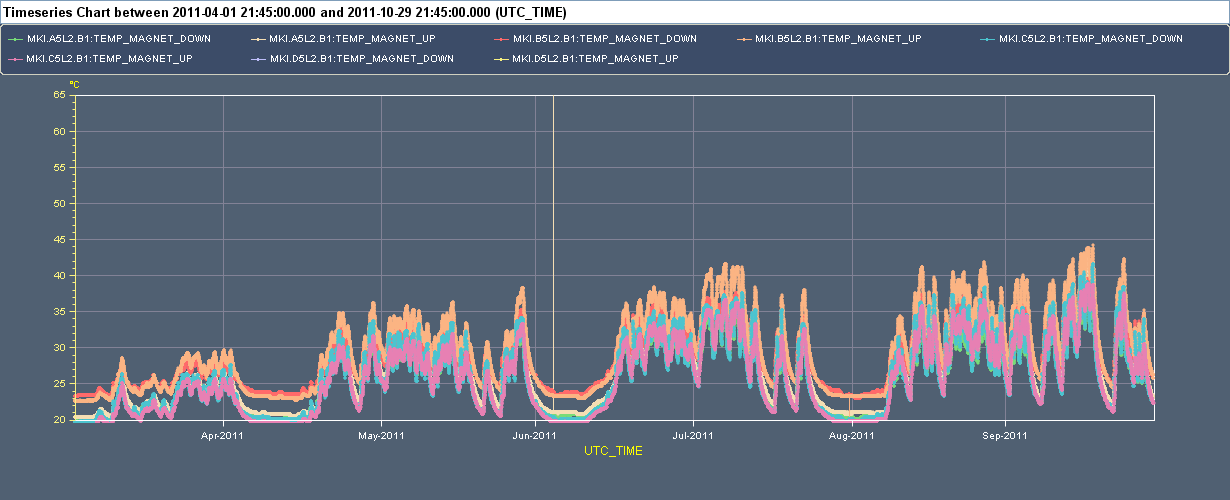
\includegraphics[width=0.85\textwidth]{LHC_MKI/figures/mkipt2_heating_before_new.png}
\label{fig:mki-ip2-heating-2011}
}
\subfigure[]{
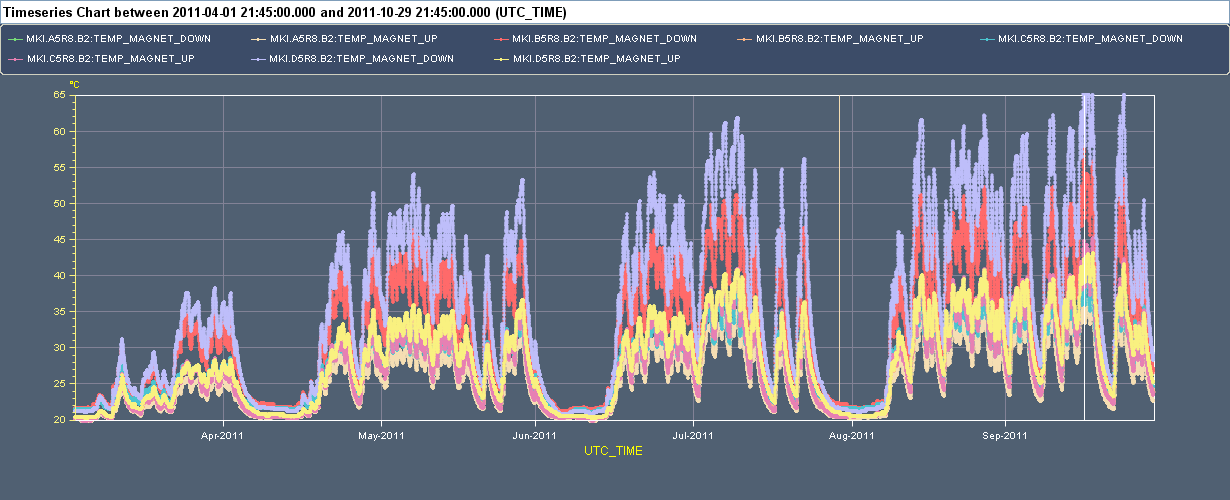
\includegraphics[width=0.85\textwidth]{LHC_MKI/figures/mkipt8_heating_before_new.png}
\label{fig:mki-ip8-heating-2011}
}
\end{center}
\label{fig:mki-heating-2011}
\caption{The heating of the MKIs at \ref{fig:mki-ip2-heating-2011} IP2 and \ref{fig:mki-ip8-heating-2011} IP8 during 2011 in the LHC. Note MKI8b and MKI8d experience significantly more heating than the other MKIs.}
\end{figure}

The temperatures in MKIs are measured using 4 PT-100 thermacouples, placed in the beam pipe up and down stream, and on the outermost ground plates up and down stream, shown in Fig.~\ref{fig:mki-thermacouple-location}. Due to the component of concern in the MKI being the ferrite yoke of the kicker but there being no direct temperature measurement on this component, one difficulty in analysing the heating of the MKI is to identify the temperature of the ferrite yoke which corresponds to which temperature at the points of measurement. This is a problem which has been analysed in depth in \cite{Barnes:mkiHeating}, in particular using field strength from kicks under a softstart condition (the firing of the magnet with no beam to inject), and inferences from both the kick strength measured in correspondance to the temperatures, and the rise time of the kicker field. Current analysis has given a certain margin of safety to the current interlock level, but due to the possible damage that may be done due to a misinjection of the beam this is very conservative, still requiring a few hours of cool down time between injections.

\begin{figure}
\label{fig:mki-thermacouple-location}
\caption{The location of the temperature measuring thermacouples in the MKI. The upstream end is towards the capactive coupling end of the beam screen.}
\end{figure}

Prior to technical stop 3 in 2012 there were 2 configurations of the beam screen in the LHC-MKIs - 7 MKIs are in place with 15 tapered screen conductors, the 9 screen conductors closest to the HV busbar having been removed due to the electrical breakdown concerns mentioned in Sec.~\ref{sec:mki-screen-development}. A single MKI, MKI8c is fitted with 24 screen conductors, 15 tapered as in the other MKIs, and 9 shortened screen conductors (trimmed such they do not overlap with the external metallization at the capacitively coupled end). This was found to reduce the induced voltage in the screen conductors closest to the HV busbar, but not significantly improve the beam coupling impedance of the MKI.